
\begin{figure*}[t] 
	\centering
	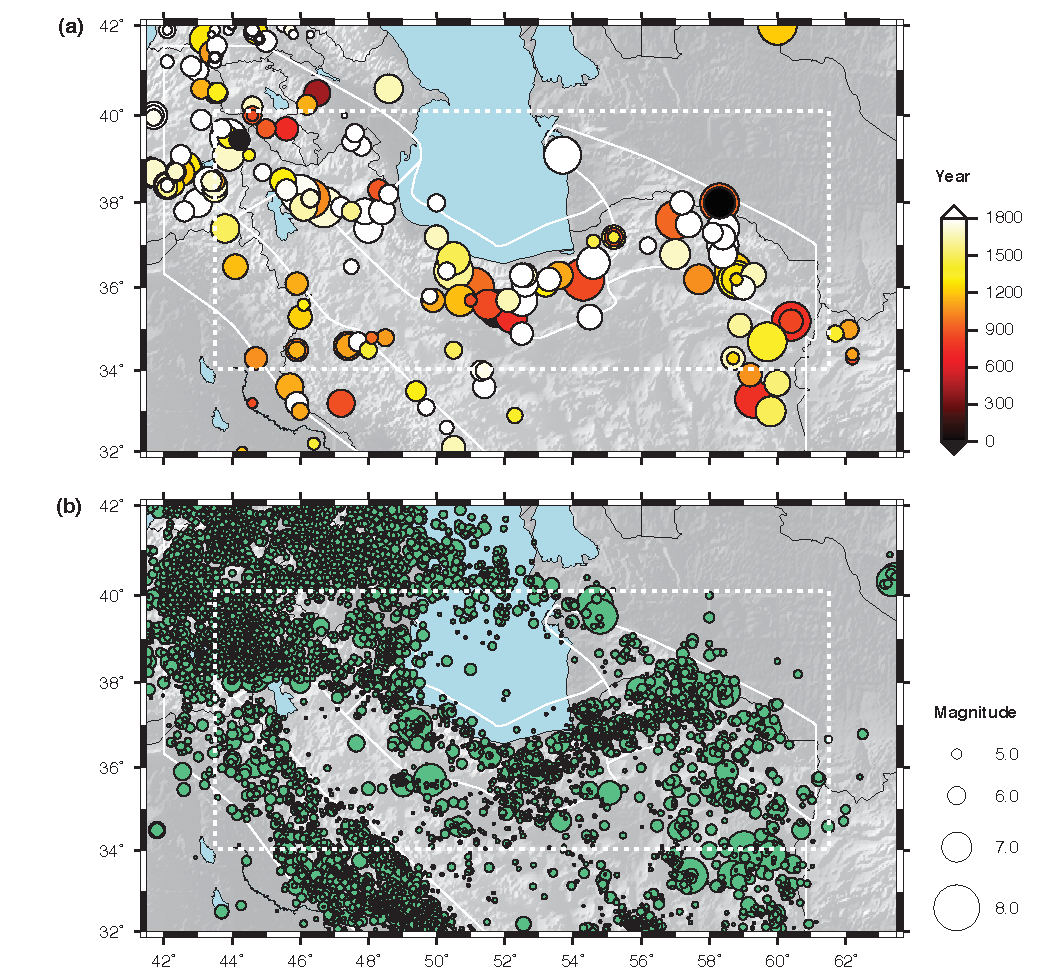
\includegraphics[width=0.9\textwidth]{figures/pdf/figure-03}
	\caption{Location of events considered in the compiled seismic catalog. (a) Historical seismicity prior to 1900 for $M_w \geq 4$ \citep[after][]{Zare2014}. (b) Instrumental seismicity up until December 2015 for $M_w \geq 3$ (IIEES) and $M_w \geq 4$ \citep[after][]{Zare2014}. Size of symbols is proportional to the magnitude of the events. In the case of the historical seismicity catalog, the color fill indicates the year of the event. The borderlines of the seismic zones shown in Fig.~\ref{fig:iran} are shown in the background in white, along with the light gray shaded relief.}
	\label{fig:catalog}
\end{figure*}

\subsection{Composition}

The first fundamental step in regional seismic hazard analysis is the composition of a reliable seismic catalog that includes both historically documented and instrumentally recorded earthquakes. Nowadays, instrumental datasets are easily accessible through international, regional, and local agencies. Historical data, on the other hand, lends itself to subjective interpretation. Notable previous efforts to compose uniform earthquake catalogs for Iran include but are not limited to \citet{Ambraseys_1982_Book}, \citet{moinfar1994}, and \citet{Berberian_1995_Tech}. These studies, however, differ from each other in their use of magnitude scales or magnitude conversion rules, and the extent to which they accept historical accounts as valid data. 

According to \citet{Ambraseys_1982_Book}, there is evidence of earthquakes as far back as the third millennium B.C., yet some of those accounts are difficult to interpret. \citet{Mirzaei1997} compiled a catalog with historical events dating back to the 4th century B.C.~and instrumental earthquakes through 1994 in which a comprehensive list of studies was considered and magnitudes uniformly converted to surface wave magnitude ($M_s$). Most ground motion prediction equations employed today in seismic hazard studies, however, use moment magnitude ($M_w$) instead. 

Recent catalogs such as that by \citet{Karimiparidari2013}, \citet{Shahvar2013}, and \citet{Zare2014} are all compiled using magnitudes converted to $M_w$. \citet{Karimiparidari2013}, for instance, compiled a catalog for Iran and adjacent areas using international and national datasets including events up until April, 2010, with $M_w > 5$. They developed relationships between moment magnitude and other magnitude scales and removed foreshocks and aftershocks using the procedure by \citet{Gardner1974}. \citet{Shahvar2013} built a catalog for the Iranian plateau for events with $M_w \geq 4$ merging data from two local and seven international datasets for the 1900--2011 period. They used the orthogonal regression method by \citet{Castellaro2006} to derive magnitude conversions and removed foreshocks and aftershocks according to the procedure by \citet{Uhrhammer_1986_EN}. In addition, \citet{Shahvar2013} provided a declustered version of the catalog. 

In this study we adopt the catalog compiled for the Middle East by \citet{Zare2014} and complement it for our particular region of interest. This catalog is particularly relevant because it is published as part of the current effort by the Global Earthquake Model (GEM) partnership and the Earthquake Model of the Middle East (EMME) project. It combines over 28 thousand records from 26 datasets with both historical and instrumental seismicity. Instrumental datasets included information from international, regional, and local agencies and networks, such as the U.S.~Geological Survey's National Earthquake Information Center (NEIC), the International Seismological Center (ISC) bulletins, the International Institute of Earthquake Engineering and Seismology (IIEES), the Iranian Seismological Center (IRSC) at the University of Tehran, and the Iranian Strong Motion Network operated by the Building and Housing Research Center (BHRC), among others. Historical data included the datasets prepared over the years by \citet{Ambraseys_1982_Book}, \citet{Ambraseys_2005_Book}, and \citet{Ambraseys_2009_Book}.

For the particular case of our region of interest, the catalog prepared by \citet{Zare2014} included events $M_w \geq 4$ between 550 B.C.~and 2006. We took information from the catalog up to December 1999, and complemented it by adding newer and more complete data from IIEES for events $M \geq 3$ between January 2000 and December 2015. While we recognize that earthquakes in the range $3 \leq M_w \leq 4$ are unlikely to cause structural damage, we include them as a means to feed the model with information about epicentral locations with potential for future larger magnitude earthquakes. By contrast, a recent seismic hazard analysis done for Iran by \citet{Khodaverdian_2016_BSSA} used a similar for events $M_w \geq 4$ catalog but only included data up until 2011, which excluded the 2012 $M_w$ 6.4 Tabriz earthquake that severely damaged the northeast part of the country.

In terms of magnitude scale, the events in \citet{Zare2014} were converted from $M_L$, $M_s$ and $m_b$ scales to $M_w$ using relationships derived by the authors and by \citet{Escordilis_2006_JS}. For consistency, we used the same conversion relationships for the portion of the catalog obtained from IIEES for $M \geq 3$ earthquakes between 2000 and 2015. The dataset from IIEES also contained events reported by ISC on a duration magnitude ($M_D$) scale. In these cases we used the empirical relationship introduced by \citet{Deniz2010} to convert $M_D$ to $M_w$. Although this relationship was derived based on a dataset for $M_w \geq 4.5$ events, we extrapolated the equation for lower magnitudes and found the results to adjust well with the general trend. 

Selection and declustering was also done in consistence with the original catalog, using the method of \citet{Gardner1974}. In summary, we obtained the whole catalog version of \citet{Zare2014}, removed the events from 2000 and forward, complemented the catalog with $M>3$ events up to 2015 from IIEES, and finally declustered the new complemented catalog removing foreshocks and aftershocks. The resulting set of events compiled for this study is shown in Fig.~\ref{fig:catalog}, which includes the spatial distribution within the region of interest for both historical and instrumental events; and in Fig.~\ref{fig:scatter}, which presents the distribution of events in time and magnitude for each of the seismic zones, as well as for the complete region of interest (hereafter referred as the uniform model).

\begin{figure*} [t]
	\centering
	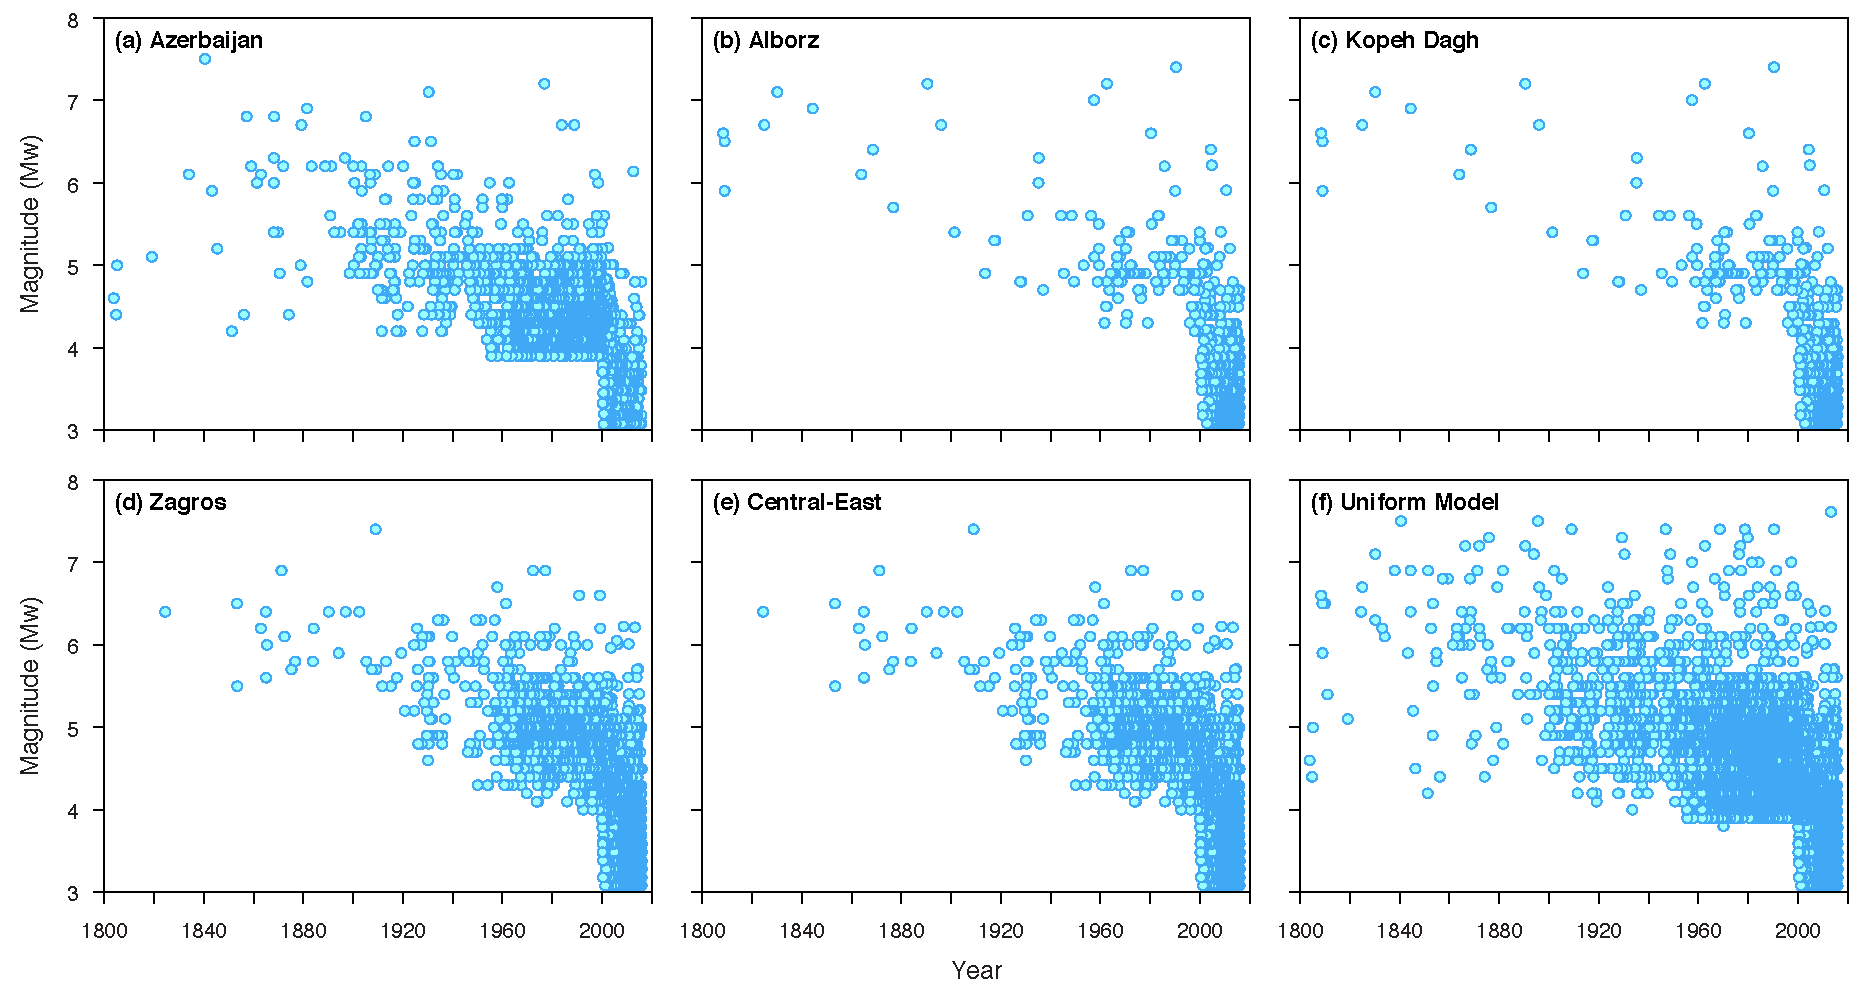
\includegraphics[width=\textwidth]{figures/pdf/figure-04}
	\caption{Magnitude-time distribution of earthquakes in each of the seismic zones, and the complete region of interests (here referred to as the uniform model).}
	\label{fig:scatter}
\end{figure*}
